\documentclass[12pt]{article}
\usepackage[a4paper,margin=1in]{geometry}
\usepackage{graphicx}
\usepackage{setspace}
\usepackage{titling}
\usepackage{ragged2e}
\usepackage{amsmath}
\usepackage{amssymb}
\usepackage{amsfonts}
\usepackage{mathtools} 

\newcommand{\course}{INF8245AE Machine Learning}
\newcommand{\assignment}{Assignment #2}
\newcommand{\university}{Polytechnique Montréal}

\begin{document}

\begin{titlepage}
    \centering
    \vspace*{1.5cm}

    {\LARGE\scshape \university \par}
    \vspace{1.5cm}

    {\Huge\bfseries \course \par}
    \vspace{1cm}

    {\Large\bfseries \assignment \par}
    \vspace{1.5cm}

    {\Huge\bfseries \titletext \par}
    \vspace{2cm}

    {\Large Ali Abbas \\ Student ID: 2078188 \par}
    \vspace{2cm}

    {\large \supervisor \par}
    \vfill

\end{titlepage}

\cleardoublepage
\pagenumbering{arabic}

\newpage

\section*{K-Nearest Neighbors}
\label{sec:knn}

\textbf{2 (a) (b):}\\
\textbf{Validation Set Results:}
\begin{enumerate}

\begin{center}
\begin{tabular}{|c|c|c|c|c|c|c|c|}
\hline
\textbf{Distance} & \textbf{k=1} & \textbf{k=2} & \textbf{k=3} & \textbf{k=4} & \textbf{k=5} & \textbf{k=10} & \textbf{k=20} \\
\hline
Euclidean & 97.12\% & 96.67\% & 97.20\% & 97.26\% & 97.19\% & 97.02\% & 96.41\% \\
\hline
Cosine & 97.50\% & 97.14\% & 97.55\% & 97.61\% & 97.60\% & 97.35\% & 97.06\% \\
\hline
\end{tabular}
\end{center}

\end{enumerate}
\textbf{Test Set Results:}
\begin{enumerate}
\textbf{Euclidean Distance:} Best $k = 3$, test accuracy: 96.81\%\\

\textbf{Cosine Distance:} Best $k = 3$, test accuracy: 97.22\%
\end{enumerate}
\textbf{Trend Commentary:}
\begin{enumerate}
Cosine distance performs better than Euclidean distance with all $k$ values. Both methods show a decline in accuracy when $k$ increases beyond the optimal values of $k=3$ or $k=4$ on the validation set, likely due to noise from distant neighbors.
\end{enumerate}
\textbf{3 (b):}\\
\textbf{Time and space complexity of the building tree:}

My implementation does the follwoing:
\begin{enumerate}
\item Select the dimension to split based on the depth
\item Sort the points using {numpy.argsort} on the selected dimension
\item Recursively build left and right subtrees
\end{enumerate}

\textbf{Time Complexity:} $O(n \log^2 n)$\\
At each level of recursion, I used \texttt{np.argsort} to find the median along the selected dimension, which requires sorting the points and takes $O(n \log n)$ time. Since the tree has a depth of $O(\log n)$ due to halving up to level k, the total time complexity becomes $O(n \log n) \times O(\log n) = O(n \log^2 n)$.

\textbf{Space Complexity:} $O(n)$
\\ At each depth of recursion I store half of the points for left and right subtrees, $n, n/2, ..., n/2^k (k = depth)$ which sums to linear space O(n).
\\\\
\textbf{3 (c):}\\
\textbf{Time complexity of traversing the tree:} $O(n)$\\
Assuming a worst case scenario where the algorithm would need to traverse from depth 0 to k the time complexity would be $O(k)$.
\\\\\textbf{3 (d):}\\
The test accuracy using the KD-tree is $100\%$
\label{sec:stone}

\subsection*{Question 4}
\begin{enumerate}
\item[(a)]
Show that for any classifier G, $R(G) = \mathbb{E}[\eta(X)1_{G(X)=0} + (1 - \eta(X))1_{G(X)=1}]$\\ where $\eta(x) = P(g = 1 | X = x)$.\\
\begin{align}
R(G) &= \mathbb{E}_{X, g \thicksim v}[1_{G(X) \neq g}]\nonumber\\
R(G) &= \mathbb{E}[\mathbb{E}[1_{G(X)\neq g} | X]] \:\: \text{(Conditional Expectation)}\\\nonumber\\
1_{G(X)\neq g} &= 1_{G(X)=0, g=1} + 1_{G(X)=1, g=0}\nonumber\\
\mathbb{E}[1_{G(X)\neq g} | X = x] &= \mathbb{E}[1_{G(X)=0, g=1} + 1_{G(X)=1, g=0} | X = x]\nonumber\\
&= P(G(X)=0, g=1 | X = x) + P(G(X)=1, g=0 | X = x)\nonumber\\
&= P(g = 1 | X = x)1_{G(X)=0} + P(g = 0 | X = x)1_{G(X)=1}\nonumber\\
&= \eta(x)1_{G(X)=0} + (1 - \eta(x))1_{G(X)=1}\nonumber\\\nonumber\\
R(G) &= \mathbb{E}[\eta(X)1_{G(X)=0} + (1 - \eta(X))1_{G(X)=1}] \:\: \text{(using equation (1))}\nonumber\\\nonumber
\end{align}

\item[(b)]
% \begin{align*}
Show that R^* := R(G^*) = \mathbb{E}[\min(\eta(X), 1 - \eta(X))]\\\\
R^* &= \mathbb{E}[\min(\eta(X), 1 - \eta(X))]\\
R^* &= \mathbb{E}[\eta(X)1_{G^*(X) = 0} + (1 - \eta(X))1_{G^*(X) = 1}]\\\\
% \end{align*}
G^*(X) = \begin{cases}
0 & \text{if } \eta(X) < 1/2\\
1 & \text{elsewhere} 
\end{cases}$\\


Suppose $\eta(X)\ge \tfrac12$, then $\eta(X)\, \mathbf{1}_{G^*(X)=0}=0$\\
and $(1-\eta(X))\, \mathbf{1}_{G^*(X)=1}=1-\eta(X)\le \eta(X)$\\
So, $\min(\eta(X), 1 - \eta(X)) = (1 - \eta(X)) \: and \: R^* = \mathbb{E}[(1 - \eta(X))]$\\\\
Suppose $\eta(X)< \tfrac12$, then $\eta(X)\, \mathbf{1}_{G^*(X)=0}=\eta(X) < 1 - \eta(X)$\\
and $(1-\eta(X))\, \mathbf{1}_{G^*(X)=1}=0$\\
So, $\min(\eta(X), 1 - \eta(X)) = \eta(X) \: and \: R^* = \mathbb{E}[\eta(X)]$\\\\
Thus, in both cases, we have : \\ $R^* = \mathbb{E}[\min(\eta(X), 1 - \eta(X))]$\\
\noindent\rule{8cm}{0.4pt}\\\\
Show that for any classifier G, $R(G) - R^* = \mathbb{E}[|2\eta(X) - 1|1_{G(X) \neq G^*(X)}]$\\

$1_{G(X)= 0} = 1 - 1_{G(X)= 1}$ and $1_{G^*(X)= 0} = 1 - 1_{G^*(X)= 1}$\\
$1_{G(X)=0} - 1_{G^*(X)=0} = 1 - 1_{G(X)=1} - 1 + 1_{G^*(X)=1} = 1_{G^*(X)=1} - 1_{G(X)=1}$
\begin{align*}
R(G) - R^* &= \mathbb{E}[|2\eta(X) - 1|1_{G(X) \neq G^*(X)}]\nonumber\\\\
&= \mathbb{E}[\eta(X)1_{G(X)=0} + (1 - \eta(X))1_{G(X)=1}]\\
&\quad- \mathbb{E}[\eta(X)1_{G^*(X)=0} + (1 - \eta(X))1_{G^*(X)=1}]\\\\
&= \mathbb{E}[\eta(X)1_{G(X)=0} - \eta(X)1_{G^*(X)=0} + (1 - \eta(X))1_{G(X)=1}\\
&\quad- (1 - \eta(X))1_{G^*(X)=1}]\\\\
&= \mathbb{E}[\eta(X)(1_{G(X)=0} - 1_{G^*(X)=0}) + (1 - \eta(X))(1_{G(X)=1} - 1_{G^*(X)=1})]\\
&= \mathbb{E}[\eta(X)(1_{G^*(X)=1} - 1_{G(X)=1}) + (1 - \eta(X))(1_{G(X)=1} - 1_{G^*(X)=1})]\\
&= \mathbb{E}[(2\eta(X) - 1)(1_{G^*(X)=1} - 1_{G(X)=1})]\\
\end{align*}

Case 1: suppose $1_{G^*(X) \neq G(X)} = 0$, then $1_{G^*(X)} = 1_{G(X)}$; $1_{G^*(X)} - 1_{G(X)} = 0$\\\\
Case 2: suppose $1_{G^*(X) \neq G(X)} = 1$\\
if $G^*(X) = 1$ and $G(X) = 0$, then G^*(X)=1  \: and \: \eta \geq 1/2$\\
\hookrightarrow 2\eta(X) -1 \geq 0$\\
\hookrightarrow (2\eta(X) - 1 )(1-0) = 2\eta(X) - 1$\\
since \eta(X) \geq 1/2, \: then \: $2\eta(X) - 1 = |2\eta(X) - 1|$\\\\
if $G^*(X) = 0$ and $G(X) = 1$, then G^*(X)=0  \: and \: \eta < 1/2$\\
\hookrightarrow 2\eta(X) -1 < 0$\\
\hookrightarrow (2\eta(X) - 1 )(0-1) = -(2\eta(X) - 1) = 1 - 2\eta(X)$\\
since \eta(X) < 1/2, \: then \: $1 - 2\eta(X) = |2\eta(X) - 1|$\\\\
Thus, in both cases, we have : \\ $R(G) - R^* = \mathbb{E}[|2\eta(X) - 1|1_{G(X) \neq G^*(X)}]$\\
% \noindent\rule{8cm}{0.4pt}\\\\
\item[(c)]
Show that ${R}(\hat{G}_n) - R^* \leq 2\mathbb{E}[|\eta(X) - \hat{\eta}_n(X)|]$.
\begin{align*}
R(\hat{G}_{n}) - R^* &= \mathbb{E}[|2\eta(X) - 1|1_{\hat{G}_{n}(X) \neq G^*(X)}]\\
&= 2\mathbb{E}[|\eta(X) - 1/2|1_{\hat{G}_{n}(X) \neq G^*(X)}]\\
	\end{align*}
G^*(X) = \begin{cases}
1 & \text{if } \eta(X) \geq 1/2\\
0 & \text{elsewhere}
\end{cases}$\\

$\hat{G}_{n}(X)$ = \begin{cases}
1 & \text{if } \hat{\eta}_n(X) \geq 1/2\\
0 & \text{elsewhere}
\end{cases}$\\

Case 1: suppose G^*(X) = 1 \: and \: \hat{G}_n(X) = 0$, then $\eta(X) \geq 1/2$ and $\hat{\eta}_n(X) < 1/2$\\
$\hookrightarrow \hat{\eta}_n(X) < 1/2 \leq \eta(X) \rightarrow |\eta(X) - \hat{\eta}_n(X)| \geq |\eta(X) - 1/2|$\\\\
Case 2: suppose \: G^*(X) = 0 \: and \: \hat{G}_n(X) = 1$, then $\eta(X) < 1/2$ and $\hat{\eta}_n(X) \geq 1/2$\\
\hookrightarrow \eta(X) < 1/2 \leq \hat{\eta}_n(X) \rightarrow |\eta(X) - \hat{\eta}_n(X)| \geq |\eta(X) - 1/2|$\\\\
\text{Thus, in both cases, we have :} $|\eta(X) - \hat{\eta}_n(X)| \geq |\eta(X) - 1/2|$
\begin{align*}
R(\hat{G}_n) - R^* &= 2\mathbb{E}[|\eta(X) - 1/2|1_{\hat{G}_n(X) \neq G^*(X)}]\\
&\leq 2\mathbb{E}[|\eta(X) - \hat{\eta}_n(X)|1_{\hat{G}_n(X) \neq G^*(X)}]\\
&\leq 2\mathbb{E}[|\eta(X) - \hat{\eta}_n(X)|]\\
\end{align*}


\end{enumerate}
\subsection*{Question 5}
\begin{enumerate}
\item[(a)]
Show that $\mathbb{E}[(\eta(x) - \hat{\eta}_n(X))^2] \leq 2\mathbb{E}[(\eta(x) - \tilde{\eta}_n(X))^2] + 2\mathbb{E}[(\tilde{\eta}_n(x) - \hat{\eta}_n(X))^2]$ 
\begin{align*}
	\eta(x) - \hat{\eta}_n(x) &= \eta(x) - \tilde{\eta}_n(X) + \tilde{\eta}_n(x) - \hat{\eta}_n(x)\\
	 &= (\eta(x) - \tilde{\eta}_n(x)) + (\tilde{\eta}_n(x) - \hat{\eta}_n(x))\\
	 (\eta(x) - \hat{\eta}_n(x))^2 &= (\eta(x) - \tilde{\eta}_n(x))^2 + (\tilde{\eta}_n(x) - \hat{\eta}_n(x))^2 \\
	 &\quad + 2(\eta(x) - \tilde{\eta}_n(x))(\tilde{\eta}_n(x) - \hat{\eta}_n(x))\\
\end{align*}
(Using $2ab \leq a^2 + b^2$)
\begin{align*}
	 2(\eta(x) - \hat{\eta}_n(x))(\hat{\eta}_n(x) - \tilde{\eta}_n(x)) &\leq (\eta(x) - \tilde{\eta}_n(x))^2 + (\tilde{\eta}_n(x) - \hat{\eta}_n(x))^2 \\
	 2(\mathbb{E}[(\eta(x) - \hat{\eta}_n(X))(\tilde{\eta}_n(X) - \hat{\eta}_n(X))]) &\leq \mathbb{E}[(\eta(x) - \tilde{\eta}_n(X))^2] + \mathbb{E}[(\tilde{\eta}_n(X) - \hat{\eta}_n(X))^2]\\
	 \mathbb{E}[(\eta(x) - \hat{\eta}_n(X))^2] &\leq \mathbb{E}[(\eta(x) - \tilde{\eta}_n(X))^2] + \mathbb{E}[(\tilde{\eta}_n(X) - \hat{\eta}_n(X))^2]\\
	 &\quad+ \mathbb{E}[(\eta(x) - \tilde{\eta}_n(X))^2] + \mathbb{E}[(\tilde{\eta}_n(X) - \hat{\eta}_n(X))^2]\\
	 &= 2\mathbb{E}[(\eta(x) - \tilde{\eta}_n(X))^2] + 2\mathbb{E}[(\tilde{\eta}_n(X) - \hat{\eta}_n(X))^2]\\
	%  \shortintertext{Using 2ab \leq a^2 + b^2}\\
	\end{align*}
\item[(b)] Show that $\mathbb{E}[(\eta(X) - \tilde{\eta}_n(X))^2] \leq \varepsilon + \mathbb{E}[\sum_{i=1}^{n} w_{n,i}(X)1_{\|X_i - X\| \geq \delta}]$.

\begin{align*}
\eta(X) - \tilde{\eta}_n(X) &= \eta(X) - \sum_{i=1}^n w_{n,i}(X) \eta(X_i)\\
&= \sum_{i=1}^n w_{n,i}(X) \eta(X) - \sum_{i=1}^n w_{n,i}(X) \eta(X_i)\\
&= \sum_{i=1}^n w_{n,i}(X)(\eta(X) - \eta(X_i))
\end{align*}

Since $\sum_{i=1}^n w_{n,i}(X) = 1$, Jensen's inequality:

\begin{align*}
(\eta(X) - \tilde{\eta}_n(X))^2 &= \Big(\sum_{i=1}^n w_{n,i}(X)(\eta(X) - \eta(X_i))\Big)^2\\
&\leq \sum_{i=1}^n w_{n,i}(X)(\eta(X) - \eta(X_i))^2\\
\mathbb{E}[(\eta(X) - \tilde{\eta}_n(X))^2] &\leq \mathbb{E}[\sum_{i=1}^n w_{n,i}(X)(\eta(X) - \eta(X_i))^2]
\\
\mathbb{E}[(\eta(X) - \tilde{\eta}_n(X))^2] &\leq \mathbb{E}[\sum_{i=1}^n w_{n,i}(X)(\eta(X) - \eta(X_i))^2 1_{\|X_i - X\| < \delta}]\\
&\quad + \mathbb{E}[\sum_{i=1}^n w_{n,i}(X)(\eta(X) - \eta(X_i))^2 1_{\|X_i - X\| \geq \delta}]
\end{align*}

$(\varepsilon, \delta)$-definition of limit: If $\eta$ is continuous, then for every $\varepsilon > 0$, there exists $\delta > 0$ such that for all $p: $\|x - p\| < \delta \Rightarrow |\eta(x) - \eta(p)| < \epsilon$\\
\begin{align*}
\mathbb{E}[(\eta(X) - \tilde{\eta}_n(X))^2] &\leq \mathbb{E}[\sum_{i=1}^n w_{n,i}(X)\varepsilon^2 1_{\|X_i - X\| < \delta}] + \mathbb{E}[\sum_{i=1}^n w_{n,i}(X) \cdot 1 \cdot 1_{\|X_i - X\| \geq \delta}]\\
&\leq \mathbb{E}[\sum_{i=1}^n w_{n,i}(X)\varepsilon^2] + \mathbb{E}[\sum_{i=1}^n w_{n,i}(X)1_{\|X_i - X\| \geq \delta}]\\
&\leq \varepsilon^2 \mathbb{E}[\sum_{i=1}^n w_{n,i}(X)] + \mathbb{E}[\sum_{i=1}^n w_{n,i}(X)1_{\|X_i - X\| \geq \delta}]\\
\mathbb{E}[(\eta(X) - \tilde{\eta}_n(X))^2] &\leq \varepsilon^2 + \mathbb{E}[\sum_{i=1}^n w_{n,i}(X)1_{\|X_i - X\| \geq \delta}]\\
&= \varepsilon + \mathbb{E}[\sum_{i=1}^{n} w_{n,i}(X)1_{\|X_i - X\| \geq \delta}] \text{ (since $\varepsilon$ can be close to null)}
\end{align*}


\item[(c)]  Show that $\mathbb{E}[(\tilde{\eta}_n(X) - \hat{\eta}_n(X))^2] = \mathbb{E}[\sum_{i=1}^{n} w_{n,i}^2(X)(g_i - \eta(X_i))^2]$\\
\begin{align*}
\tilde{\eta}_n(X) - \hat{\eta}_n(X) &= \sum_{i=1}^n w_{n,i}(X)\eta(X)  - \sum_{i=1}^n w_{n,i}(X)g_i\\
&= \sum_{i=1}^n w_{n,i}(X)(\eta(X) - g_i)\\
(\tilde{\eta}_n(X) - \hat{\eta}_n(X))^2 &= \Big(\sum_{i=1}^n w_{n,i}(X)(\eta(X) - g_i)\Big)^2\\
\mathbb{E}[(\tilde{\eta}_n(X) - \hat{\eta}_n(X))^2] &= \mathbb{E}\Big[\Big(\sum_{i=1}^n w_{n,i}(X)(\eta(X) - g_i)\Big)^2\Big]\\
\end{align*}

Because $g_i \in [0,1]$, we have $(g_i - \eta(x_i))^2 \leq 1$ \\
\begin{align*}
\mathbb{E}[\sum_{i=1}^{n} w_{n,i}^2(x)(g_i - \eta(x_i))^2] &\leq \mathbb{E}[\sum_{i=1}^{n} w_{n,i}^2(x)].
\end{align*}

with the weights, $w_{n,i}(x) \in \{1/k, 0\}$
\begin{align*}
\sum_{i=1}^{n} w_{n,i}^2(x) &= k(\frac{1}{k})^2 = \frac{1}{k}.
\end{align*}

Since $\sum_{i} w_{n,i}(x) = 1$,
\begin{align*}
\sum_{i} w_{n,i}^2(x) &\leq \max_{i} w_{n,i}(x) = \frac{1}{k}.
\end{align*}

Therefore,
\begin{align*}
\mathbb{E}[(\tilde{\eta}(x) - \hat{\eta}_n(x))^2] &\leq \mathbb{E}[\max_{i} w_{n,i}] = \frac{1}{k}.
\end{align*}

\item[(d)]

Combining parts (a) and (c):
\begin{align*}
\mathbb{E}[(\eta(x) - \hat{\eta}_n(X))^2] &\leq 2\varepsilon^2 + 2\mathbb{E}[\sum_{i=1}^{n} w_{n,i}(X)1_{\|X_i - X\| \geq \delta}] + \frac{2}{k}
\end{align*}

$k \to \infty$ and $\frac{k}{n} \to 0$ as $n \to \infty$, then:
$\frac{2}{k} \to 0$, $\mathbb{E}[\sum_{i=1}^{n} w_{n,i}(X)1_{\|X_i - X\| \geq \delta}] \to 0$ and $\varepsilon$ can be close to null.

Therefore, $\mathbb{E}[(\eta(x) - \hat{\eta}_n(X))^2] \to 0$.

\end{enumerate}



\section*{Logistic Regression}
\label{sec:logistic}
\begin{enumerate}
    \item[(a)]\\
    \textbf{Gradient with respect to W:}
\begin{align*}
\frac{\partial L}{\partial W} &= -\frac{1}{N}\sum_{i=1}^{N} \frac{\partial}{\partial W} \log P(g_i|X_i)\\
&= -\frac{1}{N}\sum_{i=1}^{N} \frac{1}{P(g_i|X_i)} \frac{\partial P(g_i|X_i)}{\partial W}\\
&= \frac{1}{N}\sum_{i=1}^{N} X_i \left(\frac{e^{W^T X_i + b}}{\sum_{j=1}^{K} e^{W_j^T X_i + b_j}} - \mathbf{1}_{g_i}\right)^T\\
&= \frac{1}{N} X^T \left(\frac{e^{WX + b}}{\sum_{j=1}^{K} e^{W_j^T X + b_j}} - Y\right)
\end{align*}

\textbf{Gradient with respect to b:}
\begin{align*}
    \frac{\partial L}{\partial b} &= -\frac{1}{N}\sum_{i=1}^{N} \frac{\partial}{\partial b} \log P(g_i|X_i)\\
    &= \frac{1}{N}\sum_{i=1}^{N} \left(\frac{e^{W^T X_i + b}}{\sum_{j=1}^{K} e^{W_j^T X_i + b_j}} - \mathbf{1}_{g_i}\right)\\
    &= \frac{1}{N}\left(\frac{e^{WX + b}}{\sum_{j=1}^{K} e^{W_j^T X + b_j}} - Y\right)
\end{align*}
(Y is the target)
\item[(e)]\\
Test Results: The best lambda is 0, and the test accuracy is: 0.9482\\
Plot: evolution of the accuracy on the validation set\\
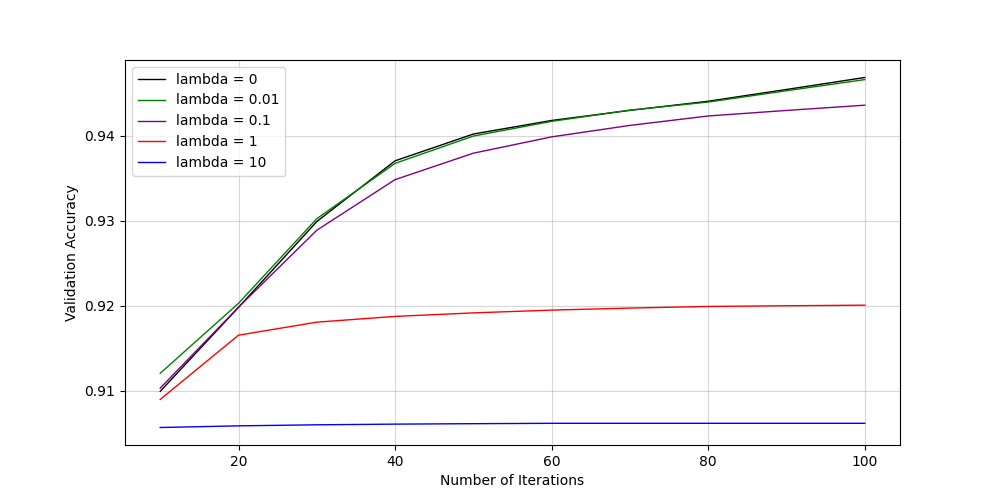
\includegraphics[width=1\textwidth]{logistic_regression_validation_accuracy.png}\\
    The lambda hyperparameter controls the strength of regularization. A higher lambda value increases the penalty on large wights, which reduces complexity and overfitting.
    According to the test results the best lambda is 0, indicating that no regularization is needed for this dataset.
    \end{enumerate}

\section*{Gaussian Naive Bayes}
\label{sec:gnb}
\begin{enumerate}
        \item[(a)]
\begin{align*}
P(g = k|X) &= \frac{P(X|g = k)P(g = k)}{P(X)}\\
\log P(g = k|X) &= \log\left(\frac{P(X|g = k)P(g = k)}{P(X)}\right)\\
&= \log P(X|g = k) + \log P(g = k) - C(X)\\
\text{where }C(X) &= \log P(X)
\end{align*}
       \item[(b)]\\
       The log-likelihood for class $k$ is:
       \begin{align*}
       \log L &= \sum_{i|g_i=k} \log P(X_i|g = k)\\
       &= \sum_{i|g_i=k} \log \mathcal{N}(X| \mu_k, \Sigma_k)\\
       &= \sum_{i|g_i=k} \left[-\frac{d}{2}\log(2\pi) - \frac{1}{2}\log|\Sigma_k| - \frac{1}{2}(X_i - \mu_k)^T\Sigma_k^{-1}(X_i - \mu_k)\right]
       \end{align*}
       
       With diagonal $\Sigma_k = \text{diag}(\sigma_1^{(k)} \ldots \sigma_d^{(k)})$:
       \begin{align*}
       \log L_k &= \sum_{i|g_i=k} \left[-\frac{d}{2}\log(2\pi) - \frac{1}{2}\sum_{j=1}^d \log(\sigma_j^{(k)})^2 - \frac{1}{2}\sum_{j=1}^d \frac{(X_{ij} - \mu_{kj})^2}{(\sigma_j^{(k)})^2}\right]
       \end{align*}
       
       \textbf{Optimizing for $\mu_k$:}
       \begin{align*}
       \frac{\partial \log L_k}{\partial \mu_{kj}} &= \sum_{i|g_i=k} \frac{X_{ij} - \mu_{kj}}{(\sigma_j^{(k)})^2} = 0\\
       \mu_{kj} &= \frac{1}{N_k}\sum_{i|g_i=k} X_{ij}\\
       \mu_k &= \frac{1}{N_k}\sum_{i|g_i=k} X_i
       \end{align*}
       
       \textbf{Optimizing for $\Sigma_k/\sigma_j$:}
       \begin{align*}
       \frac{\partial \log L_k}{\partial (\sigma_j^{(k)})^2} &= \sum_{i|g_i=k} \left[-\frac{1}{2(\sigma_j^{(k)})^2} + \frac{(X_{ij} - \mu_{kj})^2}{2((\sigma_j^{(k)})^2)^2}\right] = 0\\
       (\sigma_j^{(k)})^2 &= \frac{1}{N_k}\sum_{i|g_i=k} (X_{ij} - \mu_{kj})^2\\
       \Sigma_k &= \frac{1}{N_k}\sum_{i|g_i=k} (X_i - \mu_k)(X_i - \mu_k)^T
       \end{align*}
        \item[(e)]\\
        \textbf{GNB Test Results:}

        \textbf{MNIST Dataset:} accuracy: 74.69\%

        \textbf{IRIS Dataset:} accuracy: 100.00\%

        \textbf{Per class error rates for MNIST:}
        \begin{center}
        \begin{tabular}{|c|c|c|c|c|c|}
        \hline
        \textbf{Class} & 0 & 1 & 2 & 3 & 4 \\
        \hline
        \textbf{Error Rate} & 22.76\% & 7.22\% & 32.95\% & 54.46\% & 10.59\% \\
        \hline
        \end{tabular}
        \end{center}

        \begin{center}
        \begin{tabular}{|c|c|c|c|c|c|}
        \hline
        \textbf{Class} & 5 & 6 & 7 & 8 & 9 \\
        \hline
        \textbf{Error Rate} & 31.05\% & 11.69\% & 23.74\% & 11.29\% & 48.46\% \\
        \hline
        \end{tabular}
        \end{center}
        
        \begin{center}
        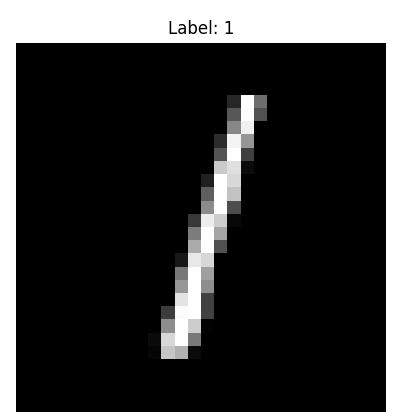
\includegraphics[width=0.3\textwidth]{class_1.png}
        \end{center}

        Class 1 has the lowest error rate (7.22\%) (highest accuracy) due to its simple vertical shape. GNB works better on IRIS (100\% accuracy) because its features are independent, while MNIST's classes (or shapes) are most likely correlated which does not fit well with GNB's assumptions. KNN outperforms GNB on MNIST by considering local patterns without distributional constraints, in other words it works best given that it has no assumptions about the distribution only about local smoothness (or the local neighborhood of points).

    \end{enumerate}

\end{document}